%%% template.tex
%%%
%%% This LaTeX source document can be used as the basis for your technical
%%% paper or abstract. Intentionally stripped of annotation, the parameters
%%% and commands should be adjusted for your particular paper - title, 
%%% author, article DOI, etc.
%%% The accompanying ``template.annotated.tex'' provides copious annotation
%%% for the commands and parameters found in the source document. (The code
%%% is identical in ``template.tex'' and ``template.annotated.tex.'')

\documentclass[conference]{acmsiggraph}

\TOGonlineid{45678}
\TOGvolume{0}
\TOGnumber{0}
\TOGarticleDOI{1111111.2222222}
\TOGprojectURL{}
\TOGvideoURL{}
\TOGdataURL{}
\TOGcodeURL{}

\title{3D Printing for Mobile Robots}

\author{Andrew Spielberg\thanks{e-mail:aespielberg@csail.mit.edu} \and Vicki Crosson\thanks{e-mail:viccro.mit@gmail.com}}
\pdfauthor{Andrew Spielberg and Vicki Crosson}



\keywords{3D Printing, Robotics, 3Doodler, Trajectory Controller}

\begin{document}

%% \teaser{
%%   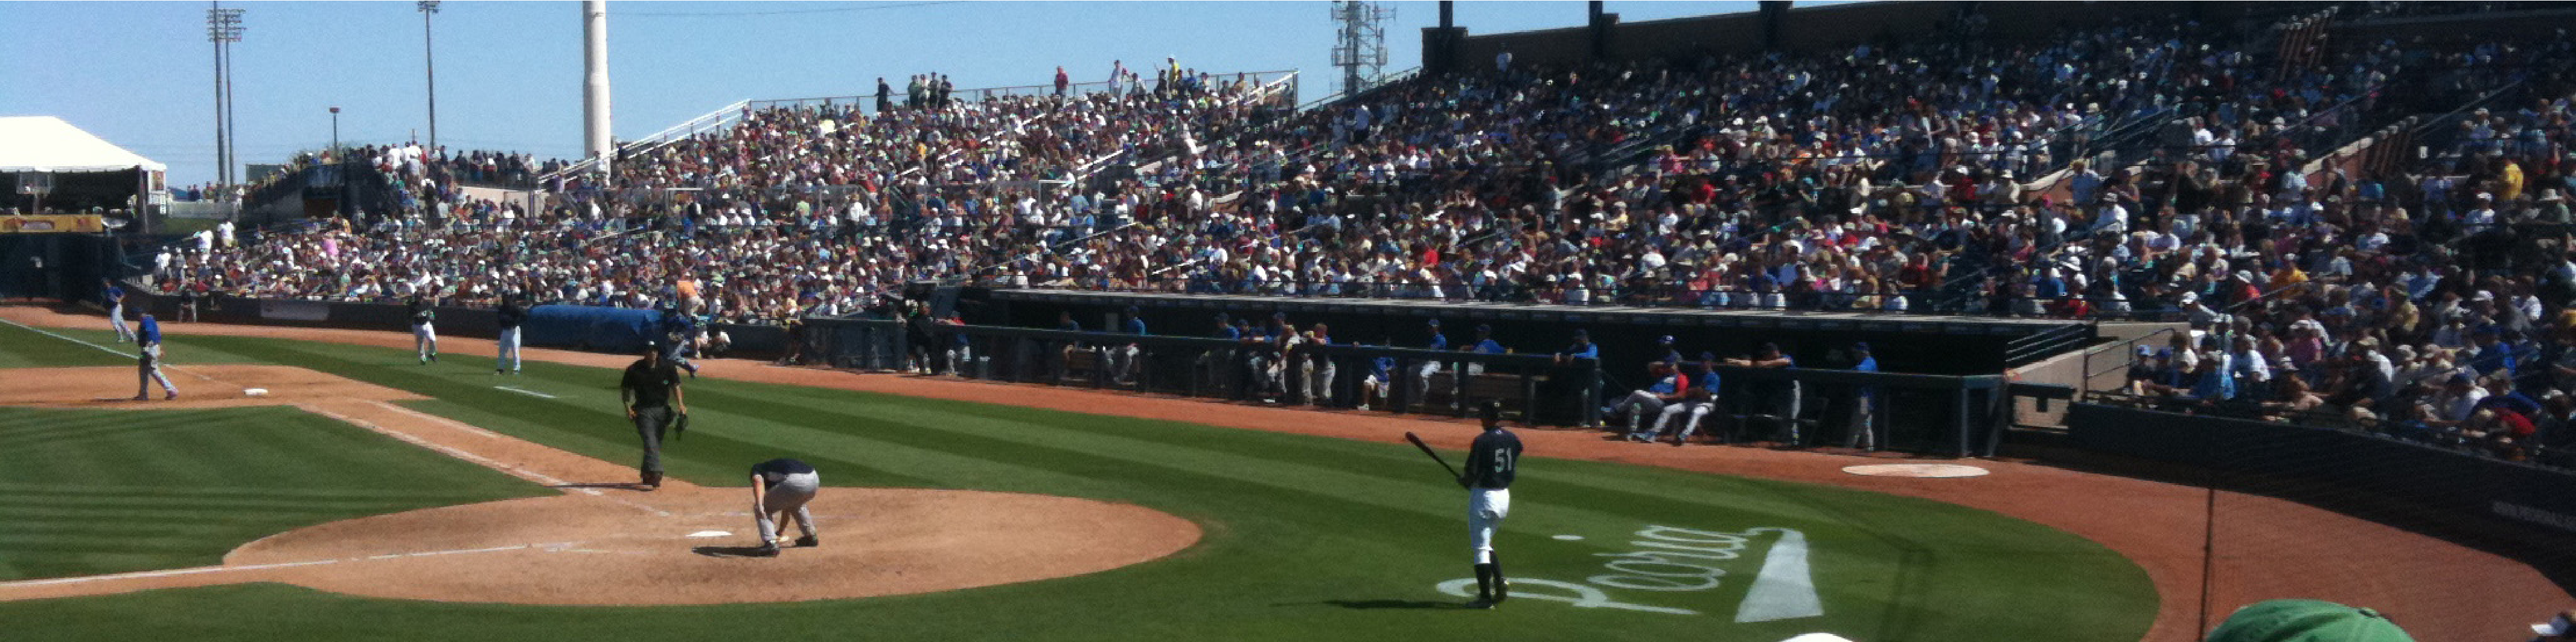
\includegraphics[height=1.5in]{images/sampleteaser}
%%   \caption{Spring Training 2009, Peoria, AZ.}
%% }

\maketitle

\begin{abstract}

Midway project report.

\end{abstract}

%\begin{CRcatlist}
%  \CRcat{I.3.3}{Computer Graphics}{Three-Dimensional %Graphics and Realism}{Display Algorithms}
%  \CRcat{I.3.7}{Computer Graphics}{Three-Dimensional %Graphics and Realism}{Radiosity};
%\end{CRcatlist}

\keywordlist

%% Use this only if you're preparing a technical paper to be published in the 
%% ACM 'Transactions on Graphics' journal.

\TOGlinkslist

%% Required for all content. 

\copyrightspace

\section{Introduction}

For our project, we seek to equip a Kuka YouBot (Figure \ref{fig:youbot}) with a plastic extruder (namely, the 3Doodler, see Figure \ref{fig:3doodler}) in order to allow a mobile manipulator to create freeform 3D shapes.  As the 3Doodler can only extrude plastic strands, all shapes that we create must be compositions of 3D curve segments.

Creating such a system requires several components, which we outline here.  In particular, the system requires:

\begin{itemize}
\item A tool for holding the 3Doodler in the youbot's fingers.
\item An electronics interface to the 3Doodler to allow it to be remotely controlled and monitored via the YouBot PC.
\item A GUI which allows users to easily create designs.
\item A tool for exporting those designs to an ordered collection of paths for the YouBot gripper to draw.
\item A velocity controller for the YouBot arm which allows for smooth extrusion in three dimensions without collisions upon previously extruded paths.
\end{itemize}

We now, in turn, discuss each of these components, their challenges, how they are currently being implemented, the remaining work which we'll aim to deliver in this class, and what will probably have to be left for future work.  Finally, we discuss our goal for our final deliverable (demonstration prints).  Throughout this project, The Robot Operating System (ROS), a commonly used framework for developing robot applications and communicating between robots on a network (and programs on a robot) is used.

Our code is being hosted on Github in a private repository, if you would like access to see our files we can add you to the repository!

\begin{figure}[ht]
  \centering
  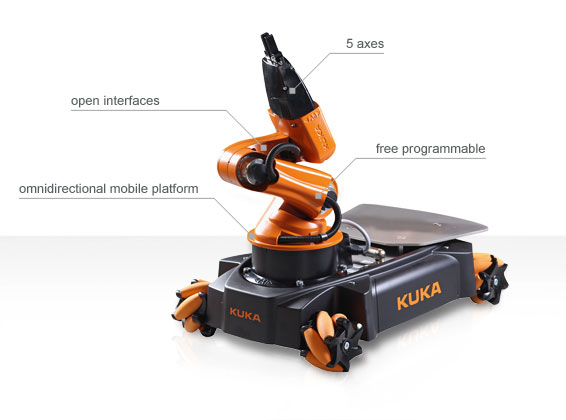
\includegraphics[width=3.0in]{images/youbot.jpg}
  \caption{The Kuka Youbot.}
  \label{fig:youbot}
\end{figure}

\begin{figure}[ht]
  \centering
  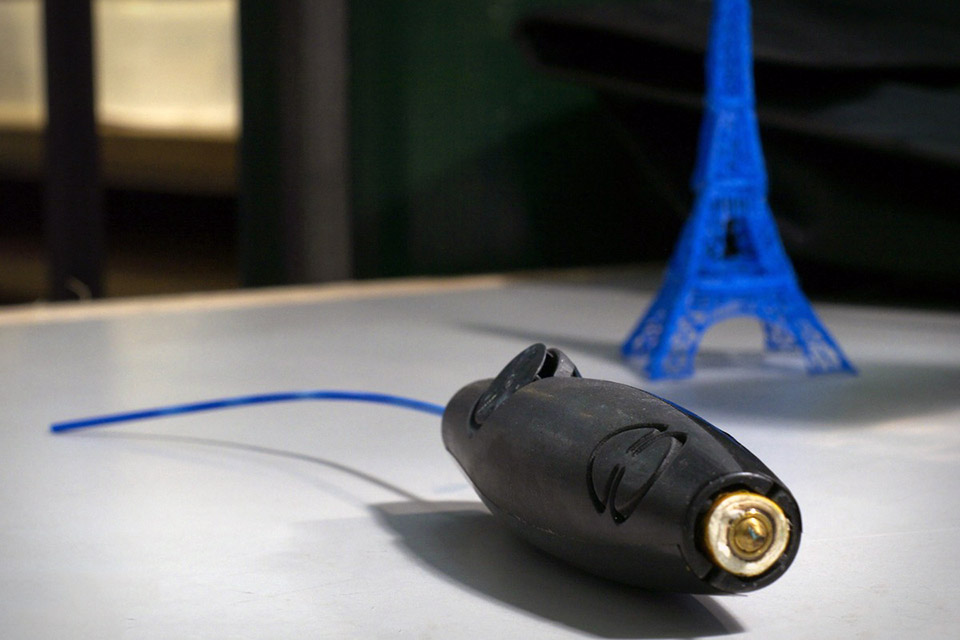
\includegraphics[width=3.0in]{images/3doodler.jpg}
  \caption{The 3Doodler Pen.}
  \label{fig:3doodler}
\end{figure}



\section{YouBot 3Doodler Clamp Tool}
We designed a 3Doodler clamp with four ideas in mind - first, that fit onto the existing gripper fingers of the YouBot so that the robot could equip and unequip it as necessary; second, that it be fabricated in two halves, so that it can be easily disassembled by us if necessary, third, that it hold the 3Doodler rigidly in place, and fourth, that it not weigh more than the YouBot's payload (1.6~kg).

In order to achieve the third point, we designed a two ringed structure which snugly fits 3Doodler geomtry at two locations, reducing the degrees of freedom to merely rotation about its extrusion axis.  Rotation here probably doesn't affect the output.  The clamp was 3D printed, and so the clamp was coated with an outer later of 0.3~mm TangoBlack+ to increase the grippiness of the clamp.

The 3Doodler initially was designed to be used with short "sticks" of ABS or PLA that the 3Doodler company sells.  Since we want to have potentially long prints without a reloading mechanism, we are feeding in material from a reel that the YouBot carries along with it.

Unfortunately, right now the 3Doodler with the clamp is too heavy, and so right now we are only using one half of the clamp (which isn't as rigid but mostly works).  We are considering shortening the clamp to reduce the weight, but we need to explore a way to do so that also leaves enough room for the plastic feed-in.

The 3Doodler Clamp was designed in openSCAD.  See figure \ref{fig:clamp} for a rendering of the design.

\begin{figure}[ht]
  \centering
  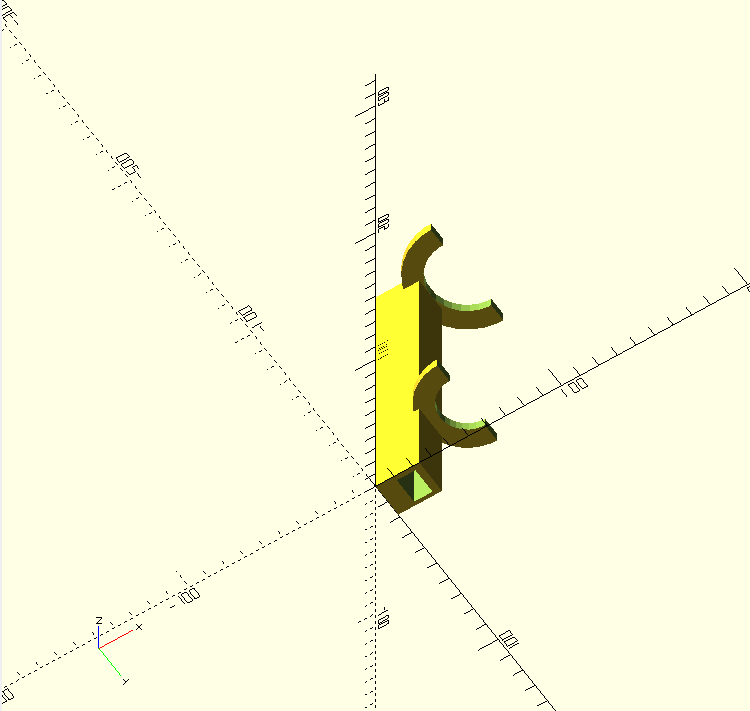
\includegraphics[width=3.0in]{images/clamp.png}
  \caption{3Doodler Clamp.}
  \label{fig:clamp}
\end{figure}


\section{Electronics for ROS-3Doodler Interfacing}
TODO: Vicki.

\section{GUI}
The GUI (See Figure \ref{fig:GUI} was designed in order to allow users to easily draw arbitrary splines.  The GUI allows for B-spline creation via cube interpolation over a series of knot points, which are created on click.  Individual splines can be deleted by selecting them and hitting the delete key, (right now, the way PythonOCC works, this deletes the grid as well).  Finally, since doodled structures must be supported, we added two features.  First, when adding a knot point, if a spline is currently selected, the added knot will snap to that spline by taking the projection to the curve.  Secondly, the first spline is always completely in the $z=0$ plane, giving future splines a reliable base to build off of.

In order to make adding knot points easier when not snapping them to existing splines (since a point on a 2D screen can correspond to an infinite number of locations along a ray in 3D), we add knot points beyond the first point of a spline to the plane uniquely defined by the first point and the camera ray as the plane's normal.

Python Open CasCADe (PythonOCC) was used as an API for designing the GUI.  In retrospect, PythonOCC might have been a bad choice, since its very bad documentation is making development a bit slower than desired, and because there are two capabilities which are less than optimally implemented, the first being the fact that deletion of a spline deletes the grid as well, and the second being that the B-spline projection metric is rather bad and that thus sometimes snapping operations give undesired results.  (Adding the capability of selecting splines also required a massive ugly hack since rendered shapes and their underlying geometric curve do not reference each other.)

As a final feature, users are able to save and output their splines to a format for the Doodler.  Rather than save entire splines, for now, we save sampled polyline approximations, since our current 3Doodler path planning algorithm can only draw straight segments.

Before we submit, we'd like to add functionality to allow users to snap knots to certain grid locations, and to orient spline segments along the Cartesian axes.  Further, we'd like to add more visual feedback when adding knot points by showing the plane in which that camera view allows users to add knots to.  As a stretch goal, we'd like to allow instant printing of splines as soon as they're drawn.

\begin{figure}[ht]
  \centering
  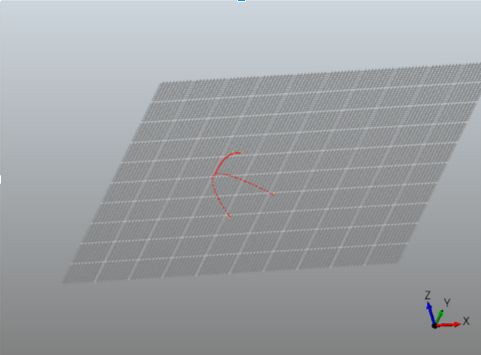
\includegraphics[width=3.0in]{images/GUI.png}
  \caption{A screenshot of the GUI with two splines.  Notice that one spline is attached to the other at a knot point.}
  \label{fig:GUI}
\end{figure}

\section{Path Ordering}
After emitting our collection of polylines from the GUI, we need to come up with a suitable order in which to draw them.  Obviously, this probably is not the order in which they are drawn, as splines can be drawn in an arbitrary order, but higher polylines cannot be fabricated before their support.  Further, in this step, we must remove any polylines which cannot be printed, namely, those suspended in mid-air with no support (if we were to add structural analysis, this could also remove any splines with bad structure).

Path ordering involves three steps.  The first step is to rescale all the polylines to a reasonable size.  For now, this is necessary because we are not using the robot base in our controller and thus are limited to a finite workspace, but when base controls are finally added, users will still want to restrict their robot to a finite sized volume on which to fabricate (note that regardless of the relaxation x and y limitations, the system will be limited in the z-axis).  The second step is to generate a constraint graph.  Polyliness must be fabricated after their support.  The final step is to order the polylines satisfying the constraint graph following a heuristic that helps to make the fabrication process as simple as possible (particularly, limiting the risk for collisions).  For now, we achieve this by preferring more "interior" polylines to be fabricated before more exterior polylines, and lower polylines before higher polylinees, in order to enforce movement in a roughly monotonic direction.  This part of the pipeline is implemented, but not currently well tested.

\section{YouBot Controller}
Control for line segments is done by smoothly interpolating between the joint configuration of a starting configuration and a target end-effector pose.  The velocity controller relies on a hand-tuned PID controller.  For now, a standard inverse kinematic solver implemented in the lab for Youbot configuration is used for computing the target arm configuration from a desired world pose.  We have also developed a velocity controller for the base, but it is unclear as of now how to integrate that into our controller planning (we consider this a stretch goal).

The arm configuration has shown the ability to consistently follow straight line trajectories.  Precision is to around 3~mm over trajectories of approximately 4~cm.  By far the greatest noise is in the z direction, which we hope to make the control smoother.  Rather than work in joint space, we may achieve this by working directly with the Jacobians of the end effector motion.  Further, we'd like to replace our current inverse kinematic solver with one which can allow us to specify "don't care" values - often, requesting a 6-DOF target for the end effector can over-constrain the IK solver and lead to target configurations with no solutions.  Having, say, a 4-DOF solver not requiring only specification of the Cartesian location in space and a target angle with the z-axis would be preferable.  Note though that this will require some caution as the direction of the 3Doodler (pushing vs. pulling) can lead to different results.  Further, we have to be careful not to self-intersect with our own drawing, so adding drawn curves to the OpenRave environment would be useful.

We also currently have an issue that the end effector is assumed to be the end of the fingers of the YouBot instead of the 3Doodler nozzle, causing wider motions than intended at the end of the nozzle.  We hope to fix this soon.  We 

\section{Demonstrations}
TODO: Vicki.  Can you also add an image of our complete Youbot setup here along with images of results?




\bibliographystyle{acmsiggraph}
\bibliography{template}
\end{document}
